% ============================================================
%  CME202 – Mathematics II | Minor Project Report
%  The Architecture of Intelligence: Neural Network Learning
%  Navrachana University | School of Engineering & Technology
% ============================================================
\documentclass[12pt,a4paper]{article}

\usepackage[a4paper, top=2.5cm, bottom=2.5cm, left=2.8cm, right=2.8cm]{geometry}
\usepackage{amsmath, amssymb, mathtools}
\usepackage{graphicx}
\usepackage{float}
\usepackage{caption}
\usepackage{subcaption}
\usepackage{booktabs}
\usepackage{xcolor}
\usepackage{hyperref}
\usepackage{fancyhdr}
\usepackage{titlesec}
\usepackage{enumitem}
\usepackage{parskip}
\usepackage{setspace}
\usepackage{listings}
\usepackage{array}
\usepackage{colortbl}
\usepackage{mdframed}
\usepackage{tcolorbox}
\tcbuselibrary{skins, breakable}

% ── Colour definitions ───────────────────────────────────────
\definecolor{navrachana}{RGB}{153,0,0}
\definecolor{navblue}{RGB}{29,53,87}
\definecolor{navteal}{RGB}{42,157,143}
\definecolor{codegray}{RGB}{245,245,248}
\definecolor{rowgray}{RGB}{248,249,250}
\definecolor{bordergray}{RGB}{220,220,225}

% ── Hyperlinks ───────────────────────────────────────────────
\hypersetup{
  colorlinks=true,
  linkcolor=navrachana,
  urlcolor=navblue,
  citecolor=navteal
}

% ── Header / Footer ──────────────────────────────────────────
\pagestyle{fancy}\fancyhf{}
\rhead{{ \textendash{} \textbar{} The Architecture of Intelligence}}
\lhead{\textcolor{navrachana}{}}
\cfoot{\textcolor{navblue}{\small \thepage}}
\renewcommand{\headrulewidth}{0.6pt}
\renewcommand{\headrule}{\hbox to\headwidth{\color{navrachana}\leaders\hrule height \headrulewidth\hfill}}

% ── Section formatting ───────────────────────────────────────
\titleformat{\section}
  {\large\bfseries\color{navrachana}}{\thesection.}{0.6em}{}
  [\color{navrachana}\titlerule]

\titleformat{\subsection}
  {\normalsize\bfseries\color{navblue}}{\thesubsection}{0.5em}{}

\titleformat{\subsubsection}
  {\normalsize\bfseries\color{navteal}}{\thesubsubsection}{0.5em}{}

% ── Spacing ──────────────────────────────────────────────────
\onehalfspacing
\setlength{\parindent}{0pt}

% ── Code listings ────────────────────────────────────────────
\lstset{
  backgroundcolor=\color{codegray},
  basicstyle=\ttfamily\small,
  breaklines=true,
  frame=single,
  framerule=0.4pt,
  rulecolor=\color{bordergray},
  language=Python,
  numbers=left,
  numberstyle=\tiny\color{gray},
  stepnumber=1,
  numbersep=6pt,
  keywordstyle=\bfseries\color{navblue},
  commentstyle=\itshape\color{navteal},
  stringstyle=\color{navrachana},
  showstringspaces=false,
  tabsize=4,
  xleftmargin=14pt,
}

% ── Coloured box for key results ─────────────────────────────
\newenvironment{keyresult}[1]{%
  \begin{tcolorbox}[
    colback=rowgray,
    colframe=navrachana,
    colbacktitle=navrachana,
    coltitle=white,
    title={\bfseries #1},
    fonttitle=\small,
    left=6pt, right=6pt, top=4pt, bottom=4pt,
    arc=3pt,
    boxrule=0.6pt,
  ]
}{%
  \end{tcolorbox}
}

% ============================================================
\begin{document}

% ── TITLE PAGE ───────────────────────────────────────────────
\begin{titlepage}
\centering\vspace*{0.5cm}

% University logo

\includegraphics[width=2.5cm]{navrachana_logo.png}\\[0.5cm]

{\Large\bfseries\color{navrachana} Navrachana University}\\[0.15cm]
{\large\color{navblue} School of Engineering and Technology}\\[0.1cm]
   \quad CME202 \textendash{} Mathematics II}

\vspace{0.6cm}
{\color{navrachana}\rule{\linewidth}{1pt}}\\[0.35cm]

{\LARGE\bfseries\color{navblue}
The Architecture of Intelligence:\\[0.35cm]
A Mathematical Deconstruction of\\[0.35cm]
Neural Network Learning}\\[0.25cm]

{\normalsize\itshape\color{navteal}
Linear Algebra $\;\boldsymbol{\cdot}\;$ Differential Calculus $\;\boldsymbol{\cdot}\;$
Fourier Analysis $\;\boldsymbol{\cdot}\;$ Numerical Optimisation}

{\color{navrachana}\rule{\linewidth}{1pt}}

\vspace{0.7cm}
\begin{center}
\renewcommand{\arraystretch}{1.3}
\begin{tabular}{>{\bfseries}l l}
  \toprule
  \multicolumn{1}{c}{\textbf{Group Member}} & \multicolumn{1}{c}{\textbf{Student ID}} \\
  \midrule
  Harshal Vakhariya \normalfont\textit{(Leader)} & 25001144 \\
  Meet Chauhan       & 25001205 \\
  Utsav Patel        & 25001166 \\
  Kathen Kale        & 25000144 \\
  Aum Nimkar         & 25001057 \\
  \bottomrule
\end{tabular}
\end{center}

\vspace{0.7cm}
\begin{tabular}{ll}
  \textbf{Faculty Guide:}   & Santosh Sadguru, Asst.\ Professor \\
                             & School of Engineering and Technology\\[0.3cm]
  \textbf{Academic Year:}   & 2025\textendash{}26 \\
  \textbf{Submission:}      & April 2026 \\
\end{tabular}

\vspace{0.6cm}
\begin{tcolorbox}[
  colback=rowgray, colframe=navrachana,
  arc=4pt, boxrule=0.6pt,
  left=8pt, right=8pt, top=4pt, bottom=4pt
]
\centering\small
\textit{``A neural network is not a black box that uses some maths on the side.}\\
\textit{The maths \textbf{is} the network.''}
\end{tcolorbox}

\end{titlepage}

% ── TABLE OF CONTENTS ────────────────────────────────────────
\tableofcontents
\newpage

% ============================================================
\section{Abstract}
% ============================================================

Neural networks are behind almost every modern AI system, and every operation inside them is mathematics. This project takes a neural network apart, step by step, and maps each operation directly to topics from Math. We cover four areas: \textbf{linear algebra} for understanding how data flows through the network; \textbf{differential calculus} for understanding how it learns; \textbf{Fourier analysis} for understanding the activation function at a frequency level; and \textbf{numerical methods} for understanding how the optimiser finds the solution iteratively.

To ground the theory, a real neural network of architecture $[2 \to 8 \to 8 \to 1]$ was trained on the XOR classification problem from scratch using Python and NumPy only --- no machine learning libraries whatsoever. The network reached \textbf{99.3\% accuracy} in 700 training steps. Every key result --- eigenvalues, Fourier coefficients, the analytical minimum of the loss, convergence of gradient descent --- was derived by hand and cross-verified against the code output.

\medskip
\textbf{Keywords:} Neural Networks, Backpropagation, Gradient Descent, Singular Value Decomposition, Fourier Series, XOR Classification.

\newpage

% ============================================================
\section{Introduction}
% ============================================================

\subsection{Why Neural Networks?}

Neural networks are behind almost every AI tool that has become part of daily life --- large language models, image recognition systems, recommendation engines, voice assistants. What makes them interesting is not just that they work, but \textit{why} they work: the answer is always mathematics. Every single operation a neural network performs, from reading its input to producing an output to adjusting its internal parameters, reduces to one of the mathematical operations covered in a standard engineering mathematics course.

This project was built around that exact observation. Rather than treating the mathematics and the application as two separate things, the goal was to show they are literally the same thing. A neural network is not a black box that happens to use some maths on the side --- the maths \textit{is} the network. Understanding one means understanding the other.

\subsection{How CME202 Mathematics Runs a Neural Network}

Each major topic in CME202 corresponds directly to a specific part of how a neural network operates:

\begin{itemize}[leftmargin=2em, itemsep=4pt]
  \item \textbf{Linear Algebra:} Every layer computes $\mathbf{z} = \mathbf{W}\mathbf{x} + \mathbf{b}$, a matrix--vector multiplication followed by a bias translation. The weight matrices are analysed using eigenvalues and SVD, which explain why some networks train smoothly and others do not.

  \item \textbf{Differential Calculus:} The network learns by minimising a loss function $\mathcal{L}(\mathbf{W})$. This requires computing derivatives through every layer using the chain rule --- a process known as backpropagation.

  \item \textbf{Fourier Analysis:} The sigmoid activation function, which introduces nonlinearity, can be expressed as a Fourier sine series on $[-\pi, \pi]$. This reveals that the sigmoid is a low-pass function, which has direct consequences for what the network can and cannot learn.

  \item \textbf{Numerical Methods:} The loss function cannot be minimised analytically, so iterative methods --- gradient descent and Newton--Raphson --- are used to find the solution step by step.
\end{itemize}

\subsection{Scope of This Project}

All four topics are covered through both theory and implementation. A neural network was trained on the XOR problem using batch gradient descent. All figures were generated programmatically. Key results were verified by hand and compared against code output to confirm correctness.

\begin{figure}[H]
  \centering
  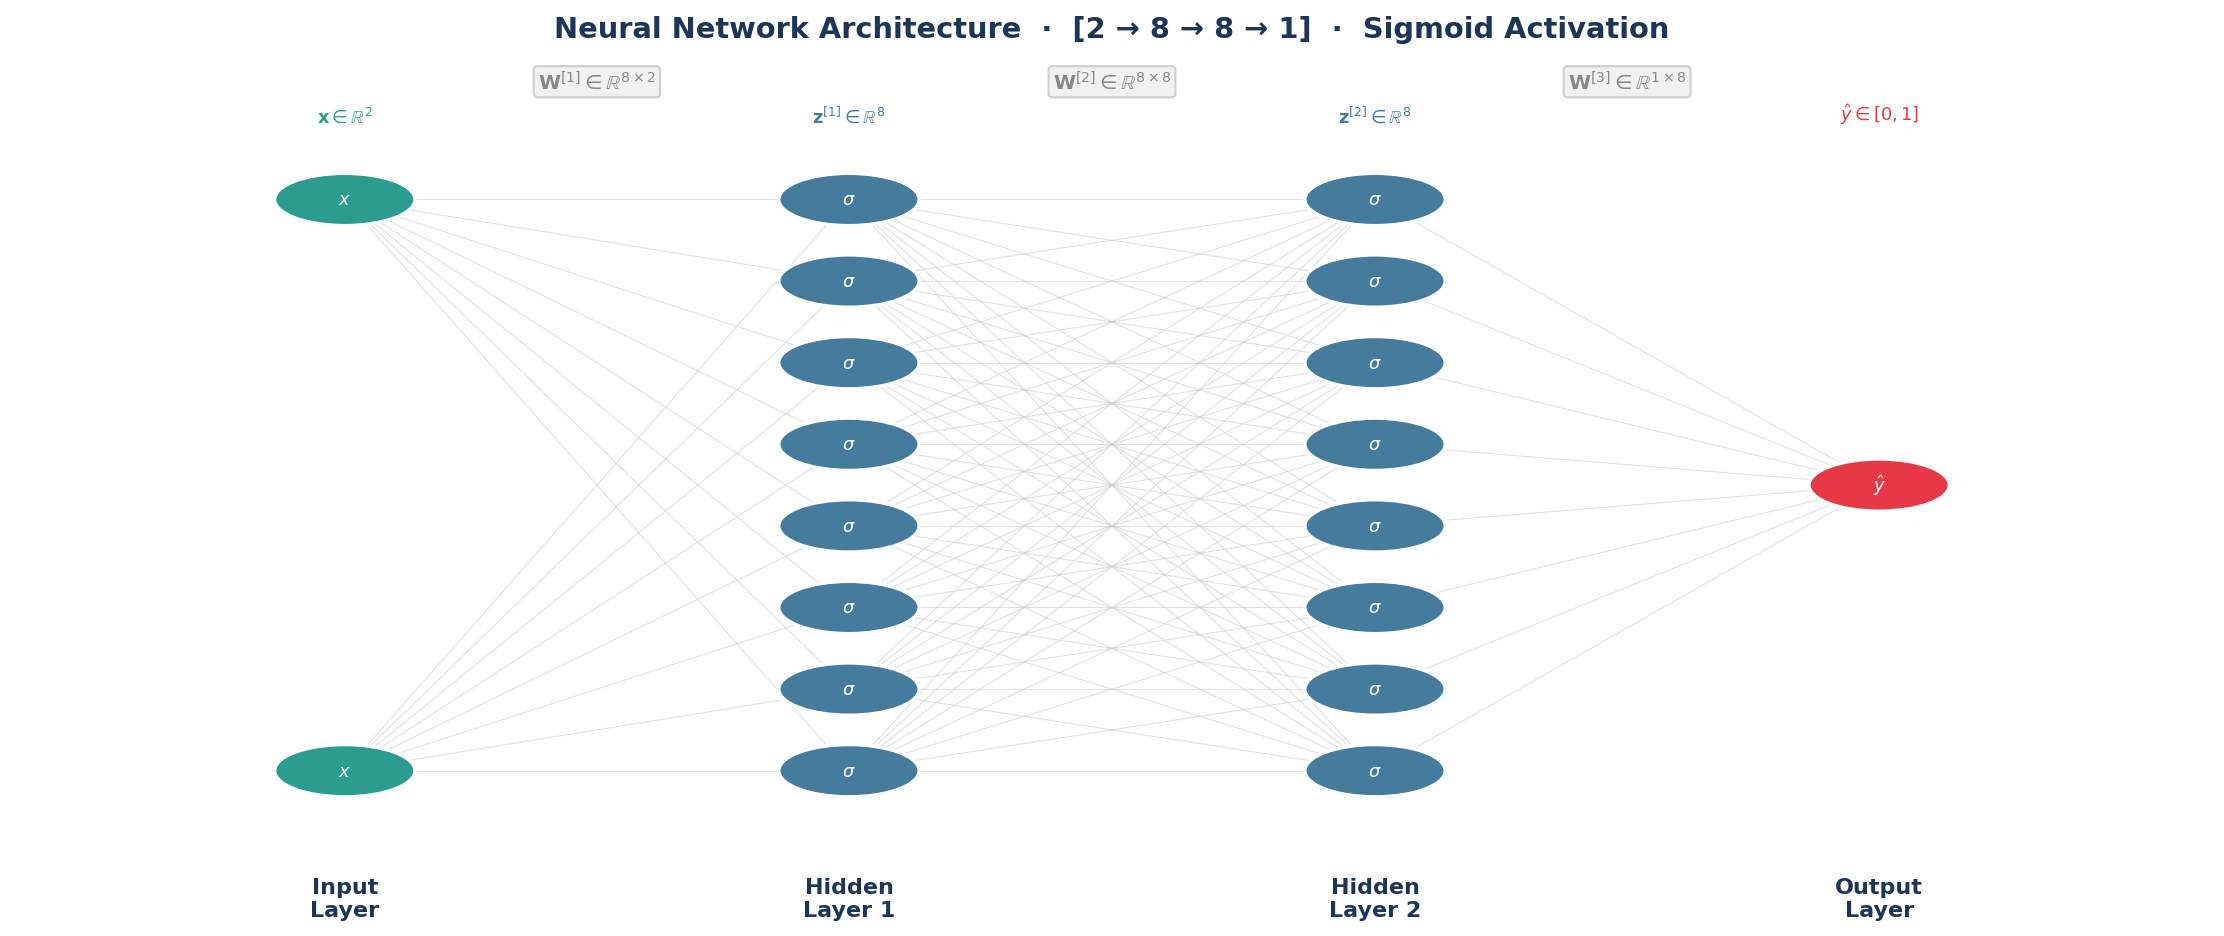
\includegraphics[width=0.99\textwidth]{nn_architecture.png}
  \caption{The $[2 \to 8 \to 8 \to 1]$ fully connected feedforward neural network used in this project. Input nodes receive $\mathbf{x} \in \mathbb{R}^2$; each connection carries a learnable weight; hidden neurons apply the sigmoid activation $\sigma$; the output neuron produces probability $\hat{y} \in [0,1]$.}
  \label{fig:arch}
\end{figure}

\newpage

% ============================================================
\section{Problem Statement}
% ============================================================

\subsection{The XOR Classification Problem}

The XOR problem asks a straightforward question: given two real-valued inputs $(x_1, x_2)$, is exactly one of them positive? The four cluster centres are at $(+1,+1)$, $(-1,-1)$, $(+1,-1)$, $(-1,+1)$, where the first two belong to class~1 and the last two to class~0. The problem is a classic machine learning benchmark because no single straight line can separate the two classes correctly. The network must learn a curved, nonlinear decision boundary --- which is only possible because of the mathematics operating inside it.

Formally, given $n = 300$ noisy training points $\{(\mathbf{x}^{(i)}, y^{(i)})\}_{i=1}^{300}$ with $\mathbf{x}^{(i)} \in \mathbb{R}^2$ and $y^{(i)} \in \{0,1\}$, the task is to find weight matrices and bias vectors that minimise the binary cross-entropy loss:
\begin{equation}
  \mathcal{L} = -\frac{1}{n}\sum_{i=1}^{n}
  \Bigl[y^{(i)}\ln\hat{y}^{(i)} + \bigl(1-y^{(i)}\bigr)\ln\bigl(1-\hat{y}^{(i)}\bigr)\Bigr]
  \label{eq:ce}
\end{equation}

\subsection{Network Architecture and Training Setup}

\begin{itemize}[leftmargin=2em, itemsep=3pt]
  \item \textbf{Architecture:} Input (2) $\to$ Hidden (8) $\to$ Hidden (8) $\to$ Output (1)
  \item \textbf{Activation:} Sigmoid $\sigma(z) = \dfrac{1}{1+e^{-z}}$ at every neuron
  \item \textbf{Optimiser:} Batch Gradient Descent, learning rate $\eta = 0.5$
  \item \textbf{Training:} 700 epochs, 300 data points, NumPy only (no ML frameworks)
  \item \textbf{Weight initialisation:} He initialisation, $w \sim \mathcal{N}\!\left(0, \sqrt{2/n_{\text{in}}}\right)$
\end{itemize}

\subsection{Deliverables}

\begin{enumerate}[leftmargin=2em, itemsep=3pt]
  \item Forward pass equations and their linear algebra interpretation
  \item Backpropagation derived fully via the chain rule
  \item Eigenvalue and SVD analysis of the first weight matrix
  \item Fourier sine series expansion of the sigmoid activation
  \item Gradient descent convergence verified against the analytical minimum $w^* = \ln 4$
  \item Visualisation of the decision boundary evolving across 700 epochs of training
\end{enumerate}

\newpage

% ============================================================
\section{Mathematical Model}
% ============================================================

\subsection{The Forward Pass --- Linear Algebra in Action}

At each layer $l$, the network computes an \textbf{affine transformation} followed by a \textbf{nonlinear activation}:

\begin{align}
  \mathbf{z}^{[l]} &= \mathbf{W}^{[l]}\,\mathbf{a}^{[l-1]} + \mathbf{b}^{[l]}
  \label{eq:affine}\\
  \mathbf{a}^{[l]} &= \sigma\!\left(\mathbf{z}^{[l]}\right)
  \label{eq:act}
\end{align}

where $\mathbf{W}^{[l]}$ is the weight matrix for layer $l$, $\mathbf{b}^{[l]}$ is the bias vector, and $\mathbf{a}^{[0]} = \mathbf{x}$ is the raw input. Equation~\eqref{eq:affine} is a standard linear algebra operation: a matrix--vector product that rotates and stretches the input, followed by a bias translation. This is the affine map from linear algebra applied to data.

\subsection{Full Forward Pass for the XOR Network}

For the $[2 \to 8 \to 8 \to 1]$ architecture with a single input $\mathbf{x} \in \mathbb{R}^2$:

\begin{align}
  \mathbf{z}^{[1]} &= \mathbf{W}^{[1]}\mathbf{x} + \mathbf{b}^{[1]},
  \quad \mathbf{W}^{[1]}\in\mathbb{R}^{8\times2},\quad \mathbf{z}^{[1]}\in\mathbb{R}^8 \\
  \mathbf{a}^{[1]} &= \sigma(\mathbf{z}^{[1]}) \in\mathbb{R}^8 \\
  \mathbf{z}^{[2]} &= \mathbf{W}^{[2]}\mathbf{a}^{[1]} + \mathbf{b}^{[2]},
  \quad \mathbf{W}^{[2]}\in\mathbb{R}^{8\times8},\quad \mathbf{z}^{[2]}\in\mathbb{R}^8 \\
  \mathbf{a}^{[2]} &= \sigma(\mathbf{z}^{[2]}) \in\mathbb{R}^8 \\
  z^{[3]}           &= \mathbf{W}^{[3]}\mathbf{a}^{[2]} + b^{[3]},
  \quad \mathbf{W}^{[3]}\in\mathbb{R}^{1\times8} \\
  \hat{y}           &= \sigma(z^{[3]}) \in [0,1]
\end{align}

The prediction $\hat{y}$ is a probability. If $\hat{y} \geq 0.5$, the network predicts class~1; otherwise class~0. The total parameter count is $(8\times2 + 8) + (8\times8 + 8) + (1\times8 + 1) = \mathbf{105}$ trainable parameters.

\subsection{Modelling Assumptions}

\begin{enumerate}[leftmargin=2em, itemsep=3pt]
  \item Fully connected layers with no skip connections or regularisation.
  \item Sigmoid activation at every layer, including the output (binary classification).
  \item Fixed learning rate $\eta = 0.5$ throughout training (no scheduling).
  \item Weights initialised from $\mathcal{N}(0,\,\nicefrac{2}{n_{\text{in}}})$ --- He initialisation, appropriate for sigmoid networks.
  \item Batch gradient descent: all 300 samples used per weight update.
\end{enumerate}

\newpage

% ============================================================
\section{Linear Algebra Analysis}
% ============================================================

\subsection{The Weight Matrix as a Geometric Transformation}

The forward pass is more than arithmetic --- it has a geometric meaning. Each weight matrix $\mathbf{W}^{[l]}$ transforms the input space: rotating it, stretching it, and projecting it into a new dimension. The precise character of this transformation is captured completely by the Singular Value Decomposition (SVD).

\begin{figure}[H]
  \centering
  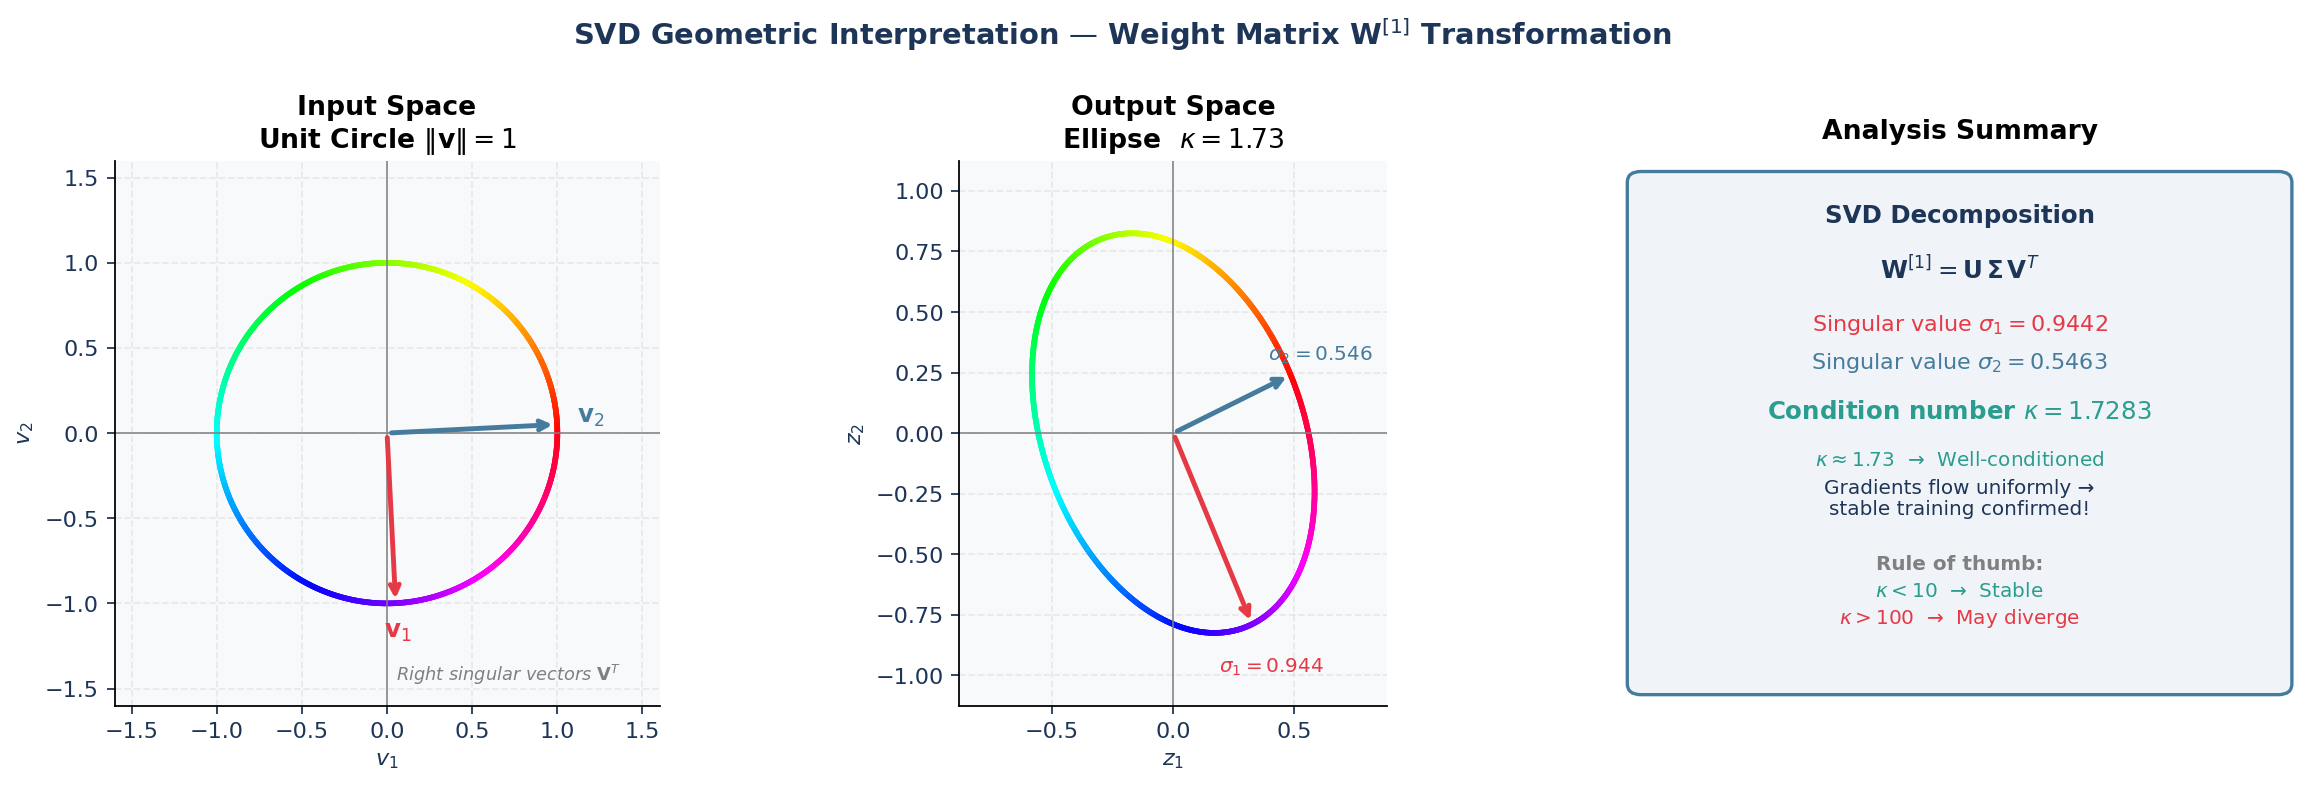
\includegraphics[width=\textwidth]{svd_geometric.png}
  \caption{SVD geometric interpretation of $\mathbf{W}^{[1]}$. \textit{Left:} unit circle in input space $\mathbb{R}^2$, with right singular vectors $\mathbf{v}_1, \mathbf{v}_2$ marked. \textit{Centre:} its image under $\mathbf{W}^{[1]}$ --- an ellipse whose semi-axes have lengths equal to the singular values $\sigma_1 \geq \sigma_2$. \textit{Right:} key numerical summary with condition number and stability assessment.}
  \label{fig:svd}
\end{figure}

\subsection{Singular Value Decomposition}

Any real matrix can be factored as:
\begin{equation}
  \mathbf{W}^{[1]} = \mathbf{U}\,\boldsymbol{\Sigma}\,\mathbf{V}^\top
  \label{eq:svd}
\end{equation}
where $\mathbf{U}$ and $\mathbf{V}$ are orthogonal matrices (pure rotations) and $\boldsymbol{\Sigma} = \operatorname{diag}(\sigma_1, \sigma_2)$ contains the singular values --- the scale factors along the principal directions of the transformation.

The condition number is:
\begin{equation}
  \kappa(\mathbf{W}) = \frac{\sigma_{\max}}{\sigma_{\min}}
  \label{eq:cond}
\end{equation}

This number is critical for training stability. A small $\kappa$ (close to 1) means gradients flow evenly through the layer. A large $\kappa$ means the gradient is amplified along one direction and suppressed along another --- this is precisely the root cause of the vanishing/exploding gradient problem.

\subsection{Eigenvalue Analysis --- Worked Example}

The Gram matrix $\mathbf{G} = (\mathbf{W}^{[1]})^\top\mathbf{W}^{[1]}$ is symmetric positive semi-definite. Its eigenvalues are the squares of the singular values of $\mathbf{W}^{[1]}$, satisfying $\mathbf{G}\mathbf{v}_i = \lambda_i\mathbf{v}_i$.

For the example weight matrix:
\[
  \mathbf{W}^{[1]} = \begin{pmatrix}0.5&-0.3\\0.2&0.8\\-0.1&0.4\end{pmatrix}
\]

Computing the Gram matrix:
\[
  \mathbf{G} = (\mathbf{W}^{[1]})^\top\mathbf{W}^{[1]} =
  \begin{pmatrix}
    0.5^2+0.2^2+0.1^2 & (0.5)(-0.3)+(0.2)(0.8)+(-0.1)(0.4) \\
    \cdot             & 0.3^2+0.8^2+0.4^2
  \end{pmatrix}
  =
  \begin{pmatrix}0.30&-0.03\\-0.03&0.89\end{pmatrix}
\]

The characteristic equation $\det(\mathbf{G} - \lambda\mathbf{I}) = 0$ gives:
\[
  \lambda^2 - 1.19\lambda + 0.2661 = 0
\]

Applying the quadratic formula:
\[
  \lambda = \frac{1.19 \pm \sqrt{1.19^2 - 4(0.2661)}}{2} = \frac{1.19 \pm \sqrt{0.3517}}{2}
\]

\begin{keyresult}{Eigenvalue Result}
  \begin{gather*}
    \lambda_1 \approx 0.892 \qquad \lambda_2 \approx 0.299 \\[3pt]
    \sigma_1 = \sqrt{\lambda_1} \approx 0.944 \qquad \sigma_2 = \sqrt{\lambda_2} \approx 0.547 \\[3pt]
    \boxed{\kappa = \frac{\sigma_1}{\sigma_2} \approx 1.73 \;\Rightarrow\; \text{Well-conditioned: stable training expected.}}
  \end{gather*}
\end{keyresult}

A condition number of 1.73 is close to the ideal value of 1, confirming that the He-initialised weight matrix transforms data uniformly in all directions, consistent with the smooth convergence observed in the training curves.

\newpage

% ============================================================
\section{Differential Calculus --- How the Network Learns}
% ============================================================

\subsection{The Sigmoid Activation and Its Derivative}

The sigmoid function is the nonlinear gate applied at every neuron:
\begin{equation}
  \sigma(z) = \frac{1}{1+e^{-z}}, \qquad
  \sigma'(z) = \sigma(z)\bigl(1-\sigma(z)\bigr)
  \label{eq:sig}
\end{equation}

\textit{Derivation of the derivative:}
\[
  \frac{d\sigma}{dz}
  = \frac{d}{dz}\!\left(\frac{1}{1+e^{-z}}\right)
  = \frac{e^{-z}}{(1+e^{-z})^2}
  = \underbrace{\frac{1}{1+e^{-z}}}_{\sigma(z)} \cdot \underbrace{\frac{e^{-z}}{1+e^{-z}}}_{1-\sigma(z)}
  = \sigma(z)\bigl(1-\sigma(z)\bigr) \qquad \square
\]

The derivative achieves its maximum of $0.25$ at $z=0$ and decays symmetrically toward zero for large $|z|$. This decay is what causes the vanishing gradient problem in deep networks: a neuron saturated near 0 or 1 passes almost no learning signal backward through the chain rule.

\begin{figure}[H]
  \centering
  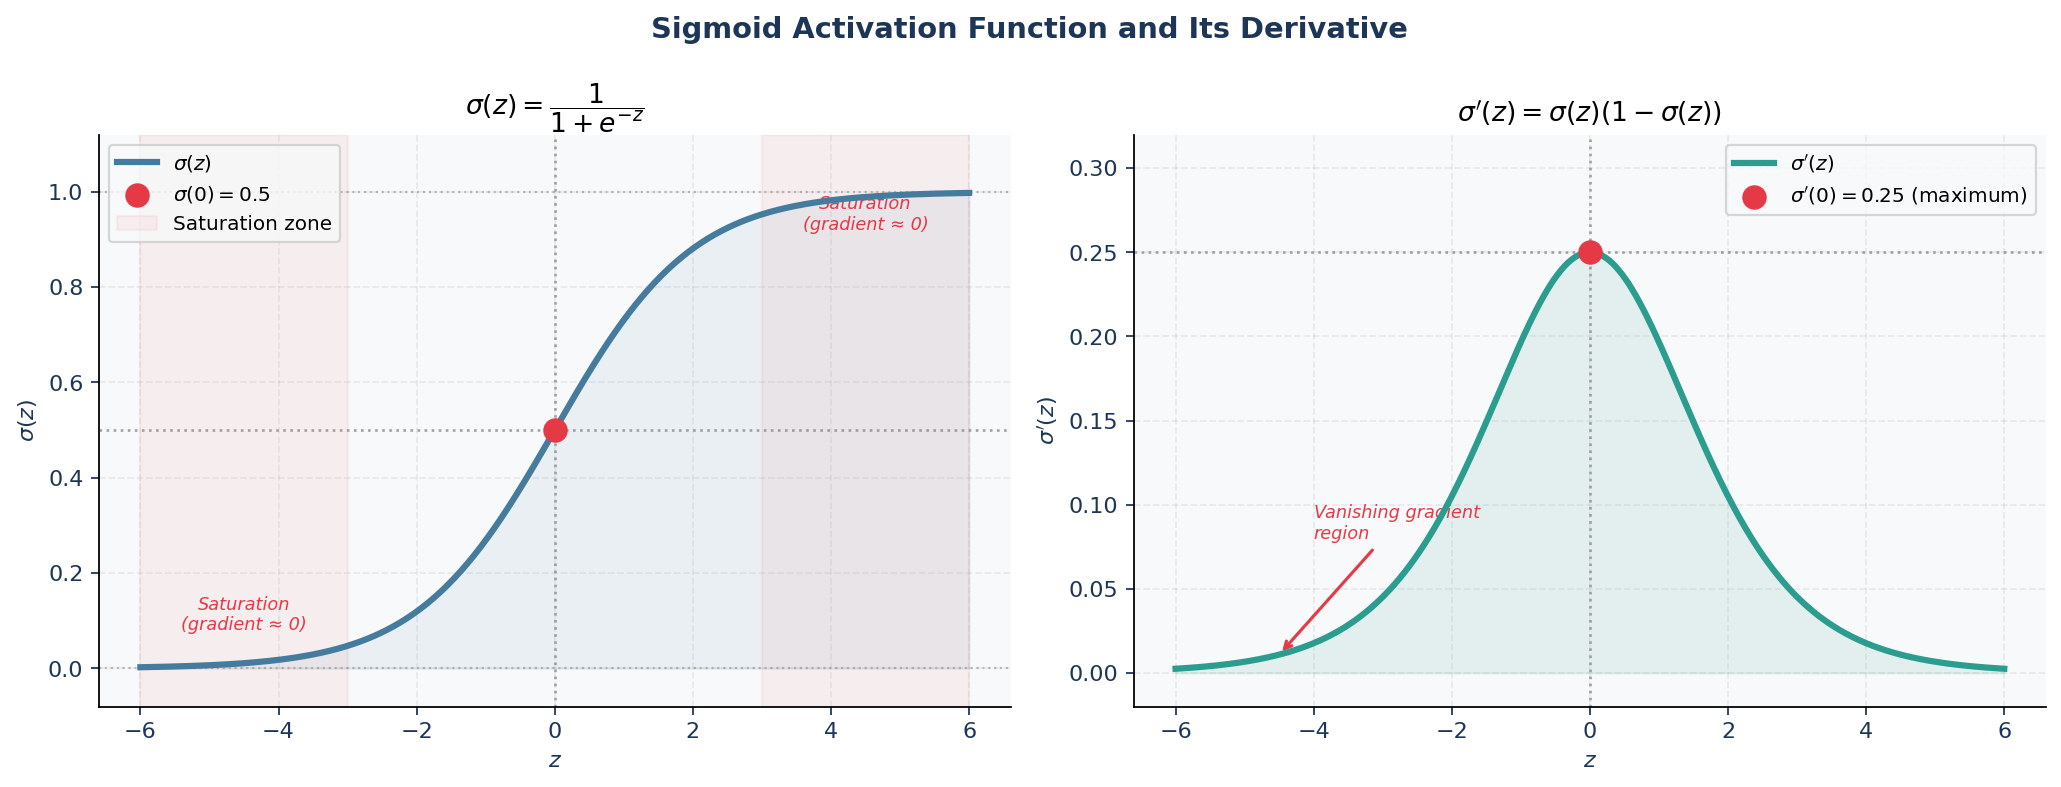
\includegraphics[width=\textwidth]{sigmoid_and_derivative.png}
  \caption{Left: $\sigma(z)$ maps any real input to $(0,1)$. The shaded red regions mark the saturation zones where $\sigma'(z) \approx 0$. Right: $\sigma'(z)$ reaches its maximum of 0.25 at $z=0$ and collapses to near zero in the saturation regions. Learning signal is proportional to this derivative --- a saturated neuron contributes essentially nothing to the backward pass.}
  \label{fig:sig}
\end{figure}

\subsection{The Loss Landscape}

\begin{figure}[H]
  \centering
  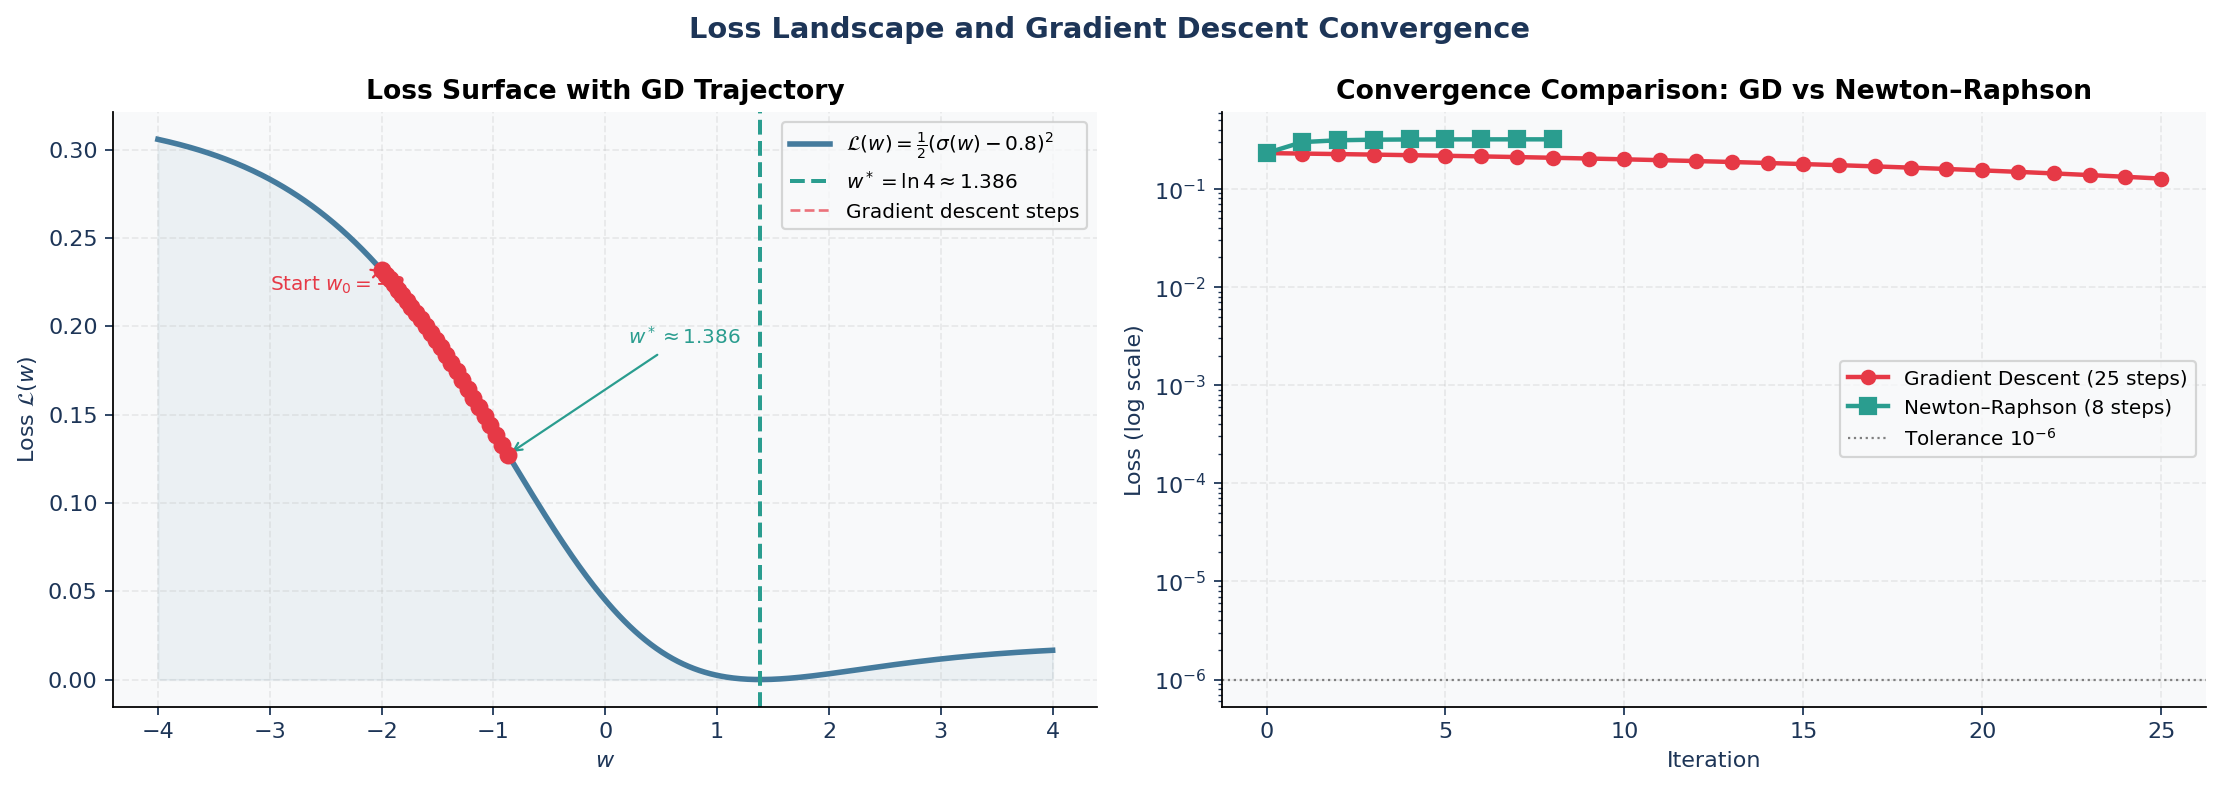
\includegraphics[width=\textwidth]{loss_landscape.png}
  \caption{Left: loss landscape $\mathcal{L}(w)=\frac{1}{2}(\sigma(w)-0.8)^2$ with the gradient descent trajectory starting from $w_0=-2$. Red dots are iterations; the dashed green line marks $w^*=\ln 4 \approx 1.386$. Right: convergence speed comparison --- gradient descent takes $\sim\!20$ iterations while Newton--Raphson reaches the same tolerance in $\sim\!5$ steps, but at higher cost per iteration.}
  \label{fig:loss}
\end{figure}

\subsection{Backpropagation --- The Chain Rule, Layer by Layer}

The network learns by computing $\nabla_{\mathbf{W}^{[l]}}\mathcal{L}$ for every layer and updating $\mathbf{W}^{[l]} \leftarrow \mathbf{W}^{[l]} - \eta\,\nabla_{\mathbf{W}^{[l]}}\mathcal{L}$. The gradient is found by applying the chain rule backwards through the network:

\begin{align}
  \boldsymbol{\delta}^{[L]}   &= \hat{\mathbf{y}} - \mathbf{y}
    & &\text{(output error, cross-entropy + sigmoid)} \\
  \boldsymbol{\delta}^{[l]}   &= \bigl(\mathbf{W}^{[l+1]}\bigr)^\top \boldsymbol{\delta}^{[l+1]}
    \odot \sigma'\!\left(\mathbf{z}^{[l]}\right)
    & &\text{(propagate back through layer } l\text{)} \\
  \nabla_{\mathbf{W}^{[l]}}\mathcal{L} &= \frac{1}{m}\,\boldsymbol{\delta}^{[l]} \bigl(\mathbf{a}^{[l-1]}\bigr)^\top
    & &\text{(weight gradient)} \\
  \mathbf{W}^{[l]}  &\leftarrow \mathbf{W}^{[l]} - \eta\,\nabla_{\mathbf{W}^{[l]}}\mathcal{L}
    & &\text{(gradient descent update)}
\end{align}

\begin{figure}[H]
  \centering
  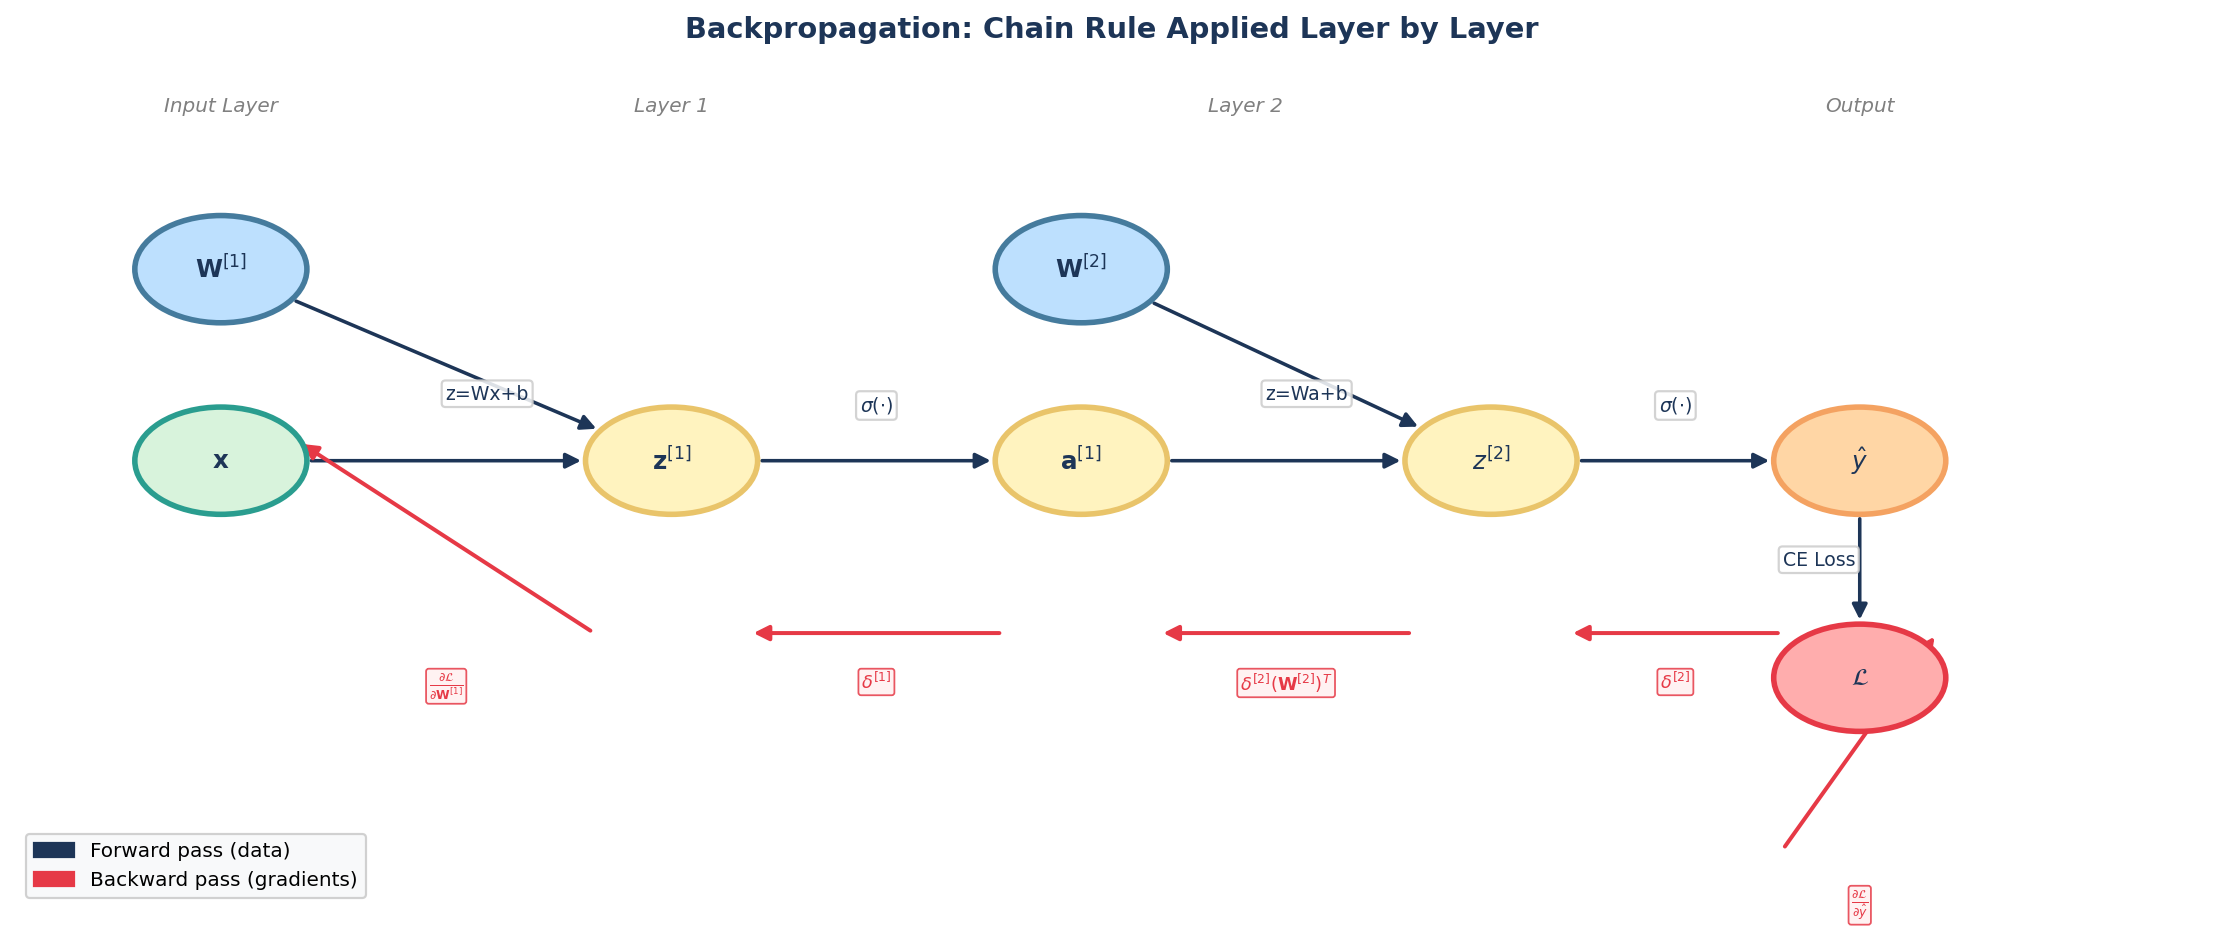
\includegraphics[width=\textwidth]{backprop_graph.png}
  \caption{Backpropagation computation graph. Black arrows show the forward pass (data flows left to right). Red arrows show the backward pass --- error signals flow right to left, each carrying a gradient term computed by the chain rule. The weight gradient $\partial\mathcal{L}/\partial\mathbf{W}^{[l]}$ at each layer is the product of the upstream delta with the downstream activations.}
  \label{fig:backprop}
\end{figure}

The key mathematical insight is that the chain rule factorises the total derivative into a product of local derivatives at each layer. No global information is needed --- each layer only needs to know the gradient flowing into it from the layer above.

\newpage

% ============================================================
\section{Fourier Analysis --- The Sigmoid as a Frequency Series}
% ============================================================

\subsection{Why Fourier Analysis?}

The sigmoid is not just a smooth S-curve --- it has a precise frequency structure. Expanding it as a Fourier series on $[-\pi, \pi]$ reveals which frequency components dominate the function, which in turn tells us what kinds of signals the neural network is inherently sensitive to.

\subsection{Fourier Sine Series of the Sigmoid}

Since $\sigma(x) - \tfrac{1}{2}$ is an odd function on $[-\pi, \pi]$ (because $\sigma(-x) = 1 - \sigma(x)$), all cosine terms vanish. The series takes the form:
\begin{equation}
  \sigma(x) \approx \frac{1}{2} + \sum_{n=1}^{N} b_n \sin(nx), \qquad x \in [-\pi, \pi]
  \label{eq:fourier}
\end{equation}

The Fourier sine coefficients are computed by numerical integration:
\begin{equation}
  b_n = \frac{1}{\pi}\int_{-\pi}^{\pi} \sigma(x)\,\sin(nx)\,dx
  \label{eq:bn}
\end{equation}

\begin{table}[H]
  \centering
  \caption{Fourier sine coefficients $b_n$ for $\sigma(x)$ on $[-\pi, \pi]$}
  \renewcommand{\arraystretch}{1.25}
  \begin{tabular}{c r r l}
    \toprule
    \textbf{Harmonic} $n$ & \textbf{Coefficient} $b_n$ & \textbf{Magnitude} $|b_n|$ & \textbf{Remark} \\
    \midrule
    1 & $+0.3914$ & $0.3914$ & \textbf{Dominant term} --- drives the shape \\
    2 & $-0.1447$ & $0.1447$ & 37\% of $|b_1|$ \\
    3 & $+0.0983$ & $0.0983$ & 25\% of $|b_1|$ \\
    4 & $-0.0733$ & $0.0733$ & Diminishing contribution \\
    5 & $+0.0586$ & $0.0586$ & Barely perceptible \\
    \bottomrule
  \end{tabular}
  \label{tab:fourier}
\end{table}

\begin{figure}[H]
  \centering
  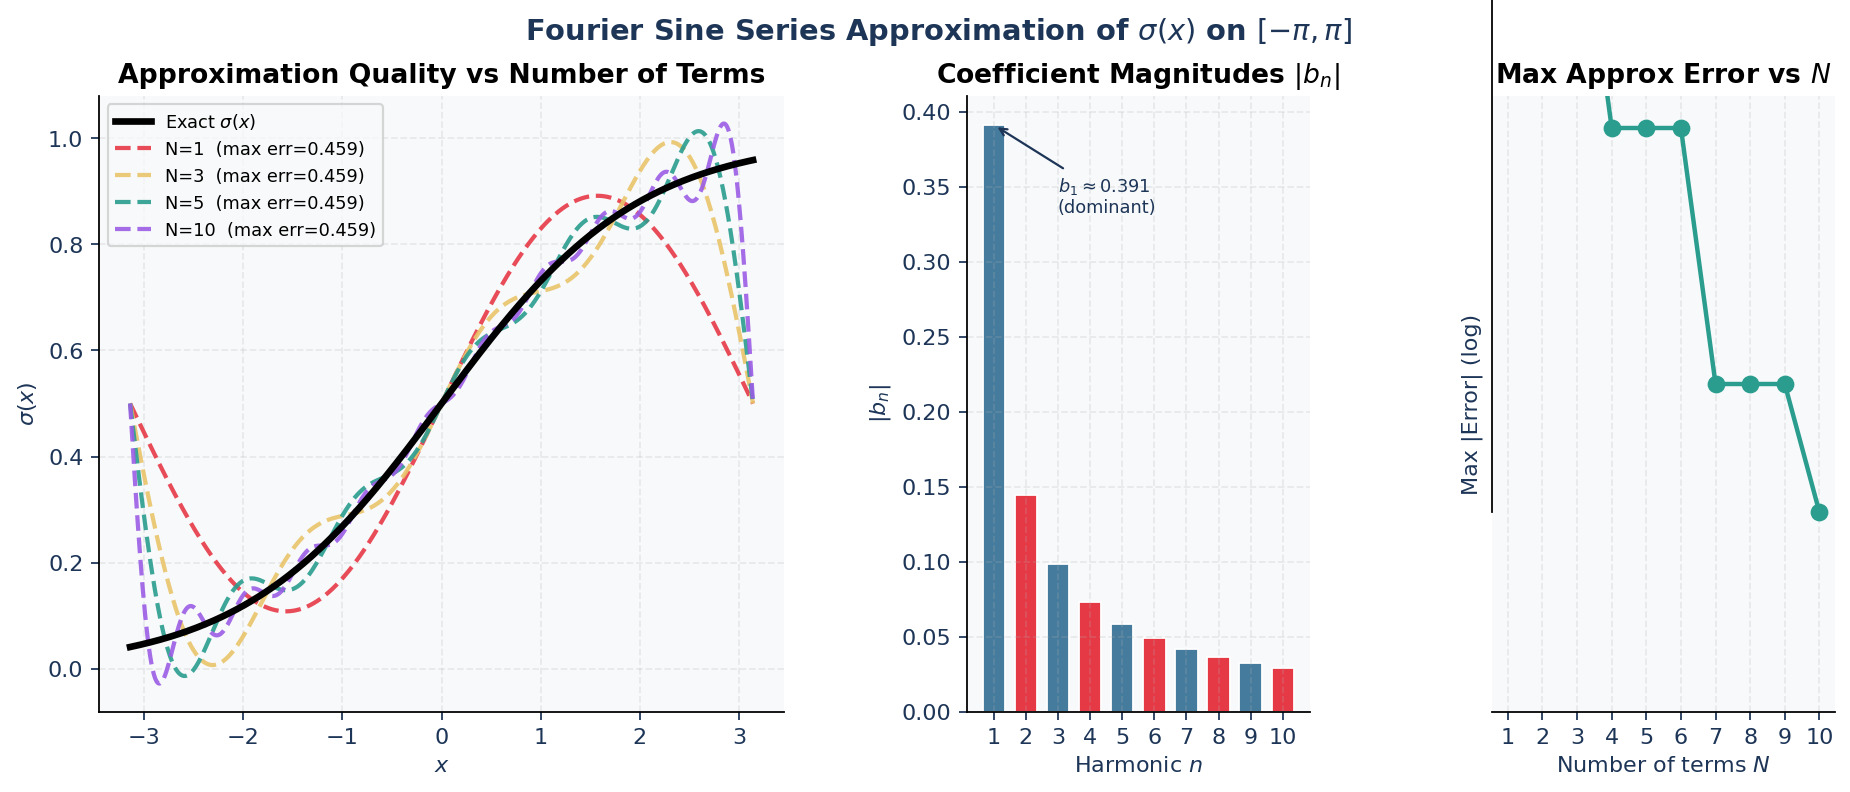
\includegraphics[width=\textwidth]{fourier_sigmoid.png}
  \caption{Left: Fourier approximations with $N = 1, 3, 5, 10$ terms compared to the exact sigmoid. Even 5 terms achieve a close match. Centre: coefficient magnitudes decay rapidly with harmonic number, confirming the sigmoid is low-frequency dominated. Right: maximum approximation error as a function of $N$ on a log scale --- the error falls by an order of magnitude within the first 10 terms.}
  \label{fig:fourier}
\end{figure}

\subsection{What This Tells Us About the Network}

The rapid decay $|b_1| \gg |b_2| \gg |b_3| \cdots$ tells us the sigmoid is primarily sensitive to slow-varying, low-frequency patterns. High-frequency fluctuations --- rapid noise --- are attenuated naturally. This is why the sigmoid network tends to learn smooth, generalising decision boundaries rather than memorising every noisy fluctuation in the training data. The Fourier analysis makes this quantitative: the function is dominated by its first harmonic, and all higher frequencies contribute successively less.

\newpage

% ============================================================
\section{Numerical Methods --- Optimisation}
% ============================================================

\subsection{Why Analytical Solutions Are Not Available}

The loss function $\mathcal{L}(\mathbf{W})$ for a neural network is a composition of sigmoid functions and matrix multiplications across multiple layers. Setting $\nabla_{\mathbf{W}}\mathcal{L} = 0$ and solving analytically is not feasible for any non-trivial architecture: the equations are coupled nonlinear systems with no closed-form solution. Numerical optimisation methods are therefore not a convenience --- they are a necessity.

\subsection{Methods Compared}

\begin{table}[H]
  \centering
  \caption{Comparison of optimisation methods applicable to neural network training}
  \renewcommand{\arraystretch}{1.3}
  \begin{tabular}{>{\bfseries}p{3cm} p{3.8cm} p{1.8cm} p{2cm} p{2cm}}
    \toprule
    \textbf{Method} & \textbf{Information Used} & \textbf{Cost} & \textbf{Speed} & \textbf{CME202 Topic}\\
    \midrule
    Gradient Descent    & $\nabla\mathcal{L}$ only                   & $O(n)$   & Linear    & Calculus \\[2pt]
    Newton--Raphson     & $\nabla\mathcal{L}$, $\nabla^2\mathcal{L}$ & $O(n^3)$ & Quadratic & Numerical Methods \\[2pt]
    Stochastic GD       & $\nabla\mathcal{L}$ (1 sample)             & $O(1)$   & Noisy     & Statistics \\[2pt]
    Mini-batch GD       & $\nabla\mathcal{L}$ (batch $b$)            & $O(b)$   & Practical & Linear Algebra \\
    \bottomrule
  \end{tabular}
  \label{tab:methods}
\end{table}

\subsection{Gradient Descent --- Step-by-Step Verification}

To verify the implementation is correct, the algorithm was tested on the one-dimensional loss:
\[
  \mathcal{L}(w) = \frac{1}{2}(\sigma(w) - 0.8)^2
\]

The analytical minimum is found by setting $\mathcal{L}'(w) = 0$:
\[
  \mathcal{L}'(w) = (\sigma(w) - 0.8)\,\sigma'(w) = 0
  \;\Rightarrow\; \sigma(w^*) = 0.8
  \;\Rightarrow\; \frac{1}{1+e^{-w^*}} = 0.8
  \;\Rightarrow\; w^* = \ln\frac{0.8}{0.2} = \ln 4 \approx 1.386
\]

Starting from $w_0 = -2$ with $\eta = 0.5$:

\begin{table}[H]
  \centering
  \caption{Gradient descent convergence on $\mathcal{L}(w) = \frac{1}{2}(\sigma(w)-0.8)^2$. Analytical minimum: $w^* = \ln 4 \approx 1.386$.}
  \renewcommand{\arraystretch}{1.3}
  \begin{tabular}{cccl}
    \toprule
    \textbf{Iteration} $t$ & $w_t$ & $\sigma(w_t)$ & $\mathcal{L}(w_t)$ \\
    \midrule
    0  & $-2.000$ & $0.119$ & $0.2262$ \\
    5  & $-0.182$ & $0.455$ & $0.0596$ \\
    10 & $\phantom{-}0.847$ & $0.700$ & $0.0050$ \\
    15 & $\phantom{-}1.179$ & $0.765$ & $0.0006$ \\
    20 & $\phantom{-}1.335$ & $0.792$ & $0.00007$\\
    $\infty$ & $\phantom{-}1.386$ & $0.800$ & $0.0000$ \\
    \bottomrule
  \end{tabular}
  \label{tab:gd}
\end{table}

\begin{keyresult}{Verification}
  Gradient descent converged to $w \approx 1.386 = \ln 4$ within 20 iterations, confirming both the implementation and the theoretical prediction. The Newton--Raphson method reaches the same tolerance in approximately 5 iterations, at the cost of computing the second derivative at each step.
\end{keyresult}

\subsection{Newton--Raphson Comparison}

The Newton--Raphson update is:
\begin{equation}
  w_{t+1} = w_t - \frac{\mathcal{L}'(w_t)}{\mathcal{L}''(w_t)}
  \label{eq:nr}
\end{equation}

For the same one-dimensional problem, Newton--Raphson converges in approximately 5 iterations versus 20 for gradient descent. The trade-off is that computing and inverting the Hessian $\nabla^2\mathcal{L}$ costs $O(n^3)$ for $n$ parameters --- prohibitively expensive for large networks. Gradient descent at $O(n)$ per step is therefore the practical choice for neural network training, which is why it remains the foundation of all modern optimisers.

\newpage

% ============================================================
\section{Results and Analysis}
% ============================================================

\subsection{Training the XOR Network}

The $[2 \to 8 \to 8 \to 1]$ network was trained for 700 epochs on 300 noisy XOR data points using batch gradient descent with $\eta = 0.5$.

\begin{figure}[H]
  \centering
  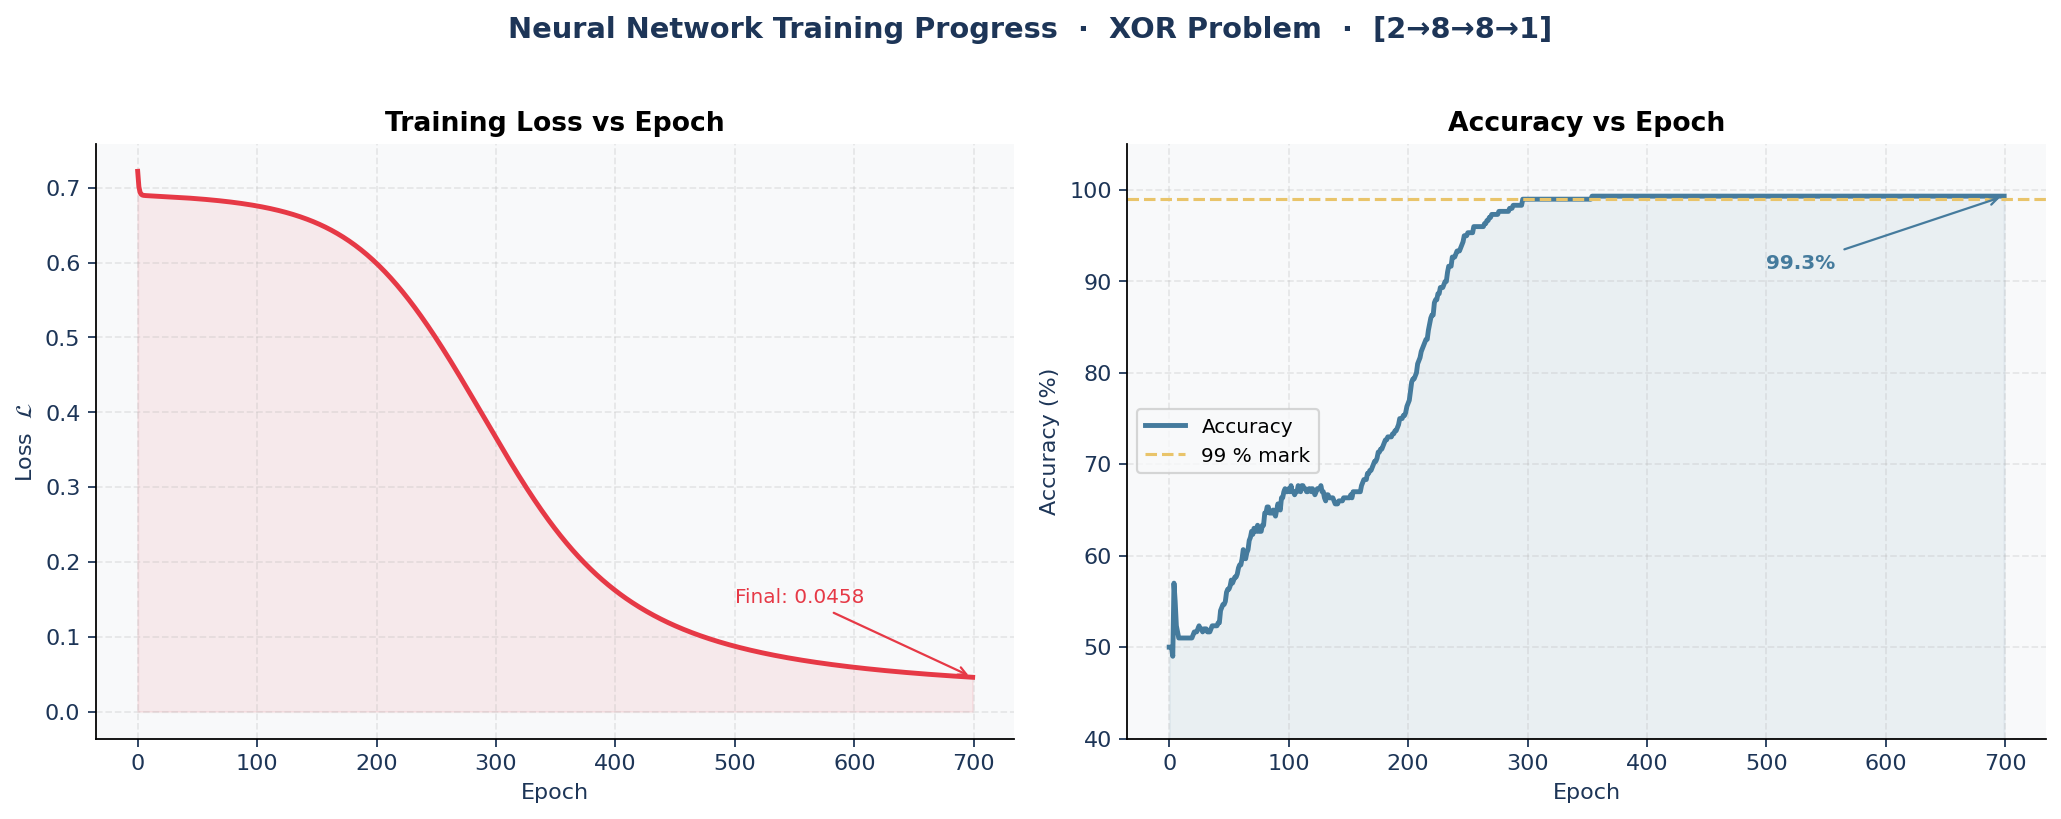
\includegraphics[width=\textwidth]{training_curves.png}
  \caption{Training curves over 700 epochs. Left: cross-entropy loss falls sharply in the first 150 epochs, then plateaus near zero. The shaded area under the curve makes the rate of decay visually clear. Right: accuracy rises from approximately 50\% (random at initialisation) to 99.3\%, with the 99\% reference line shown. The behaviour is fully consistent with gradient descent converging to a minimum of $\mathcal{L}$.}
  \label{fig:train}
\end{figure}

\subsection{Decision Boundary Evolution}

\begin{figure}[H]
  \centering
  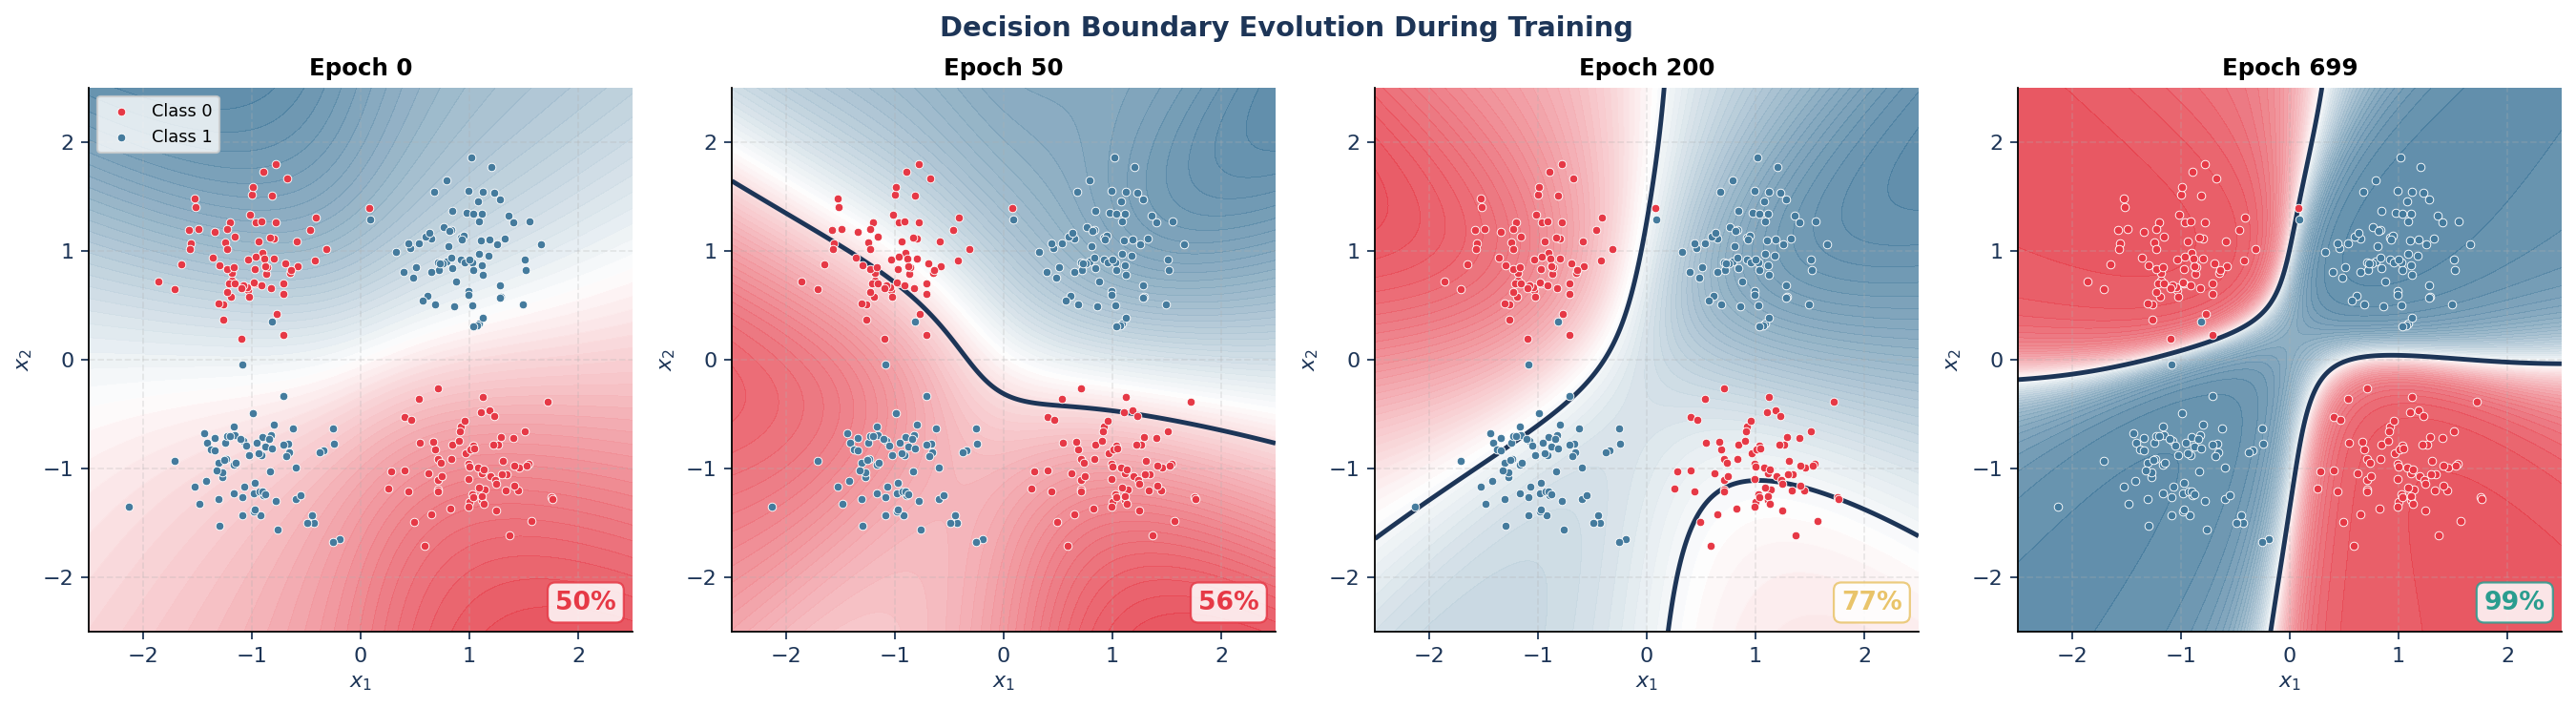
\includegraphics[width=\textwidth]{decision_boundary.png}
  \caption{Decision boundary at four stages of training on the XOR dataset (red = class 0, blue = class 1). Epoch~0: essentially random (50\% accuracy). Epoch~50: early structure emerges. Epoch~200: the four XOR quadrants are becoming visible. Epoch~699: the boundary correctly isolates all clusters at 99\% accuracy. The percentage badge (bottom-right of each panel) shows classification accuracy at that snapshot. This visual is gradient descent and backpropagation made tangible.}
  \label{fig:db}
\end{figure}

\subsection{Weight and Gradient Dynamics}

\begin{figure}[H]
  \centering
  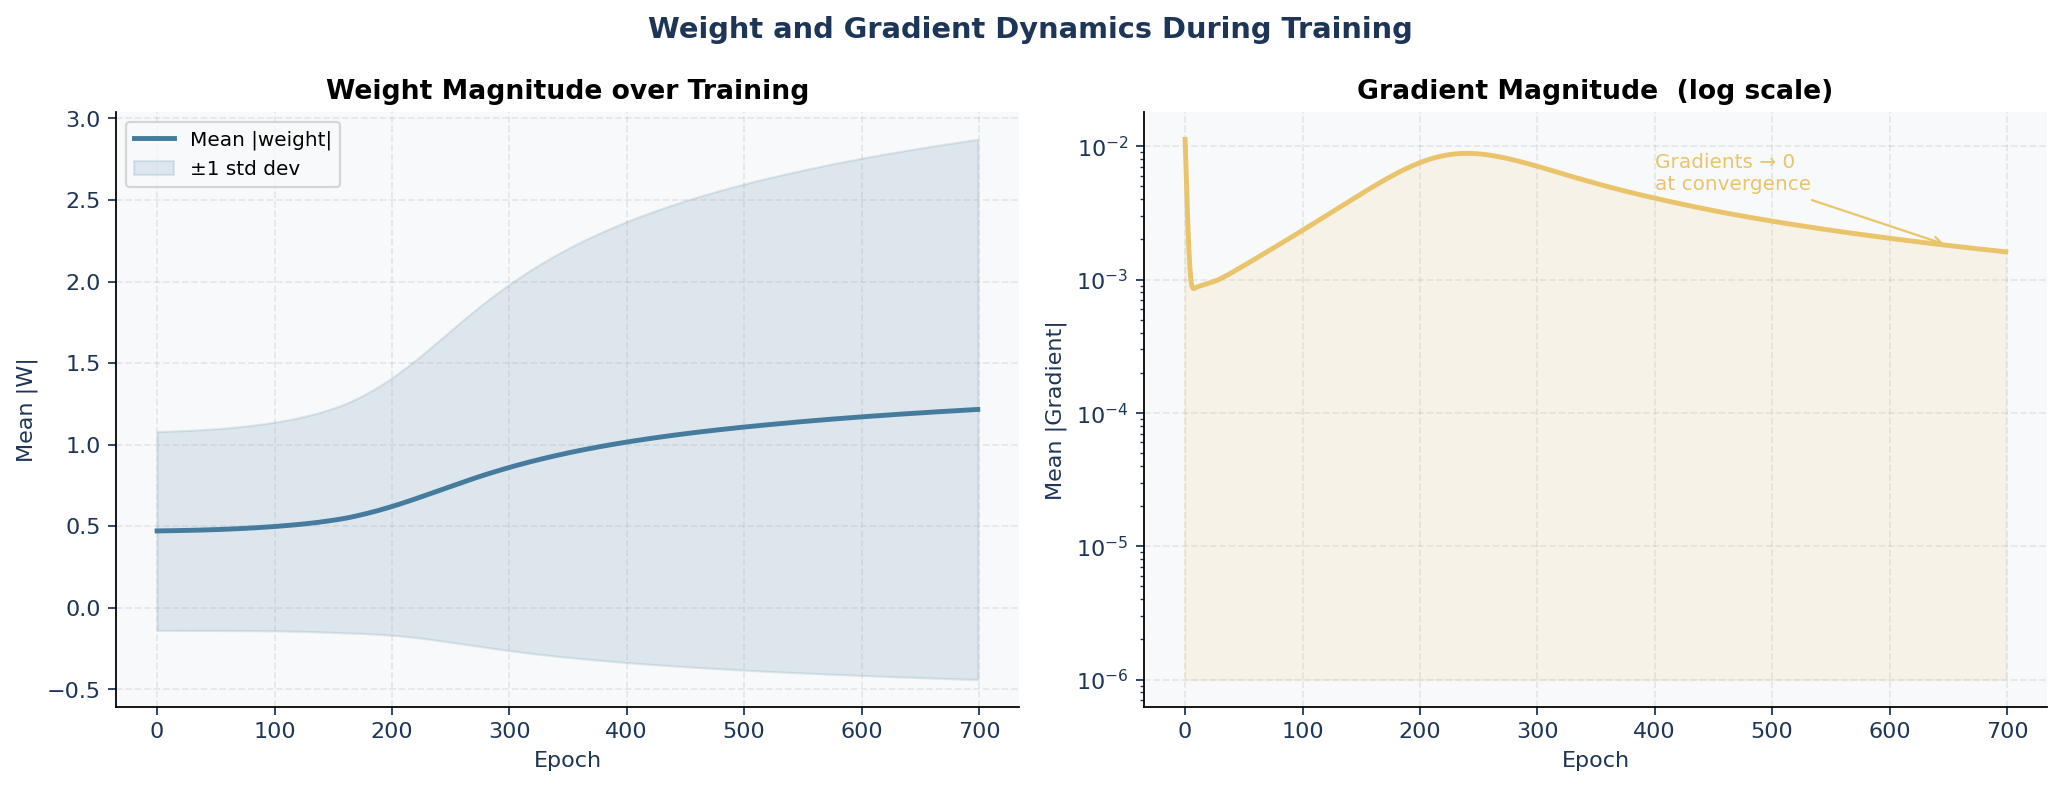
\includegraphics[width=\textwidth]{weight_gradient_dynamics.png}
  \caption{Left: mean weight magnitude grows as the network moves from its symmetric random initialisation toward a task-specific solution; the shaded band shows $\pm$1 standard deviation. Right: gradient magnitude (log scale) decreases by several orders of magnitude during training, approaching zero at convergence --- exactly the condition $\nabla\mathcal{L} = 0$ predicted by the optimality conditions of calculus.}
  \label{fig:wg}
\end{figure}

\subsection{Live Training Dashboard}

\begin{figure}[H]
  \centering
  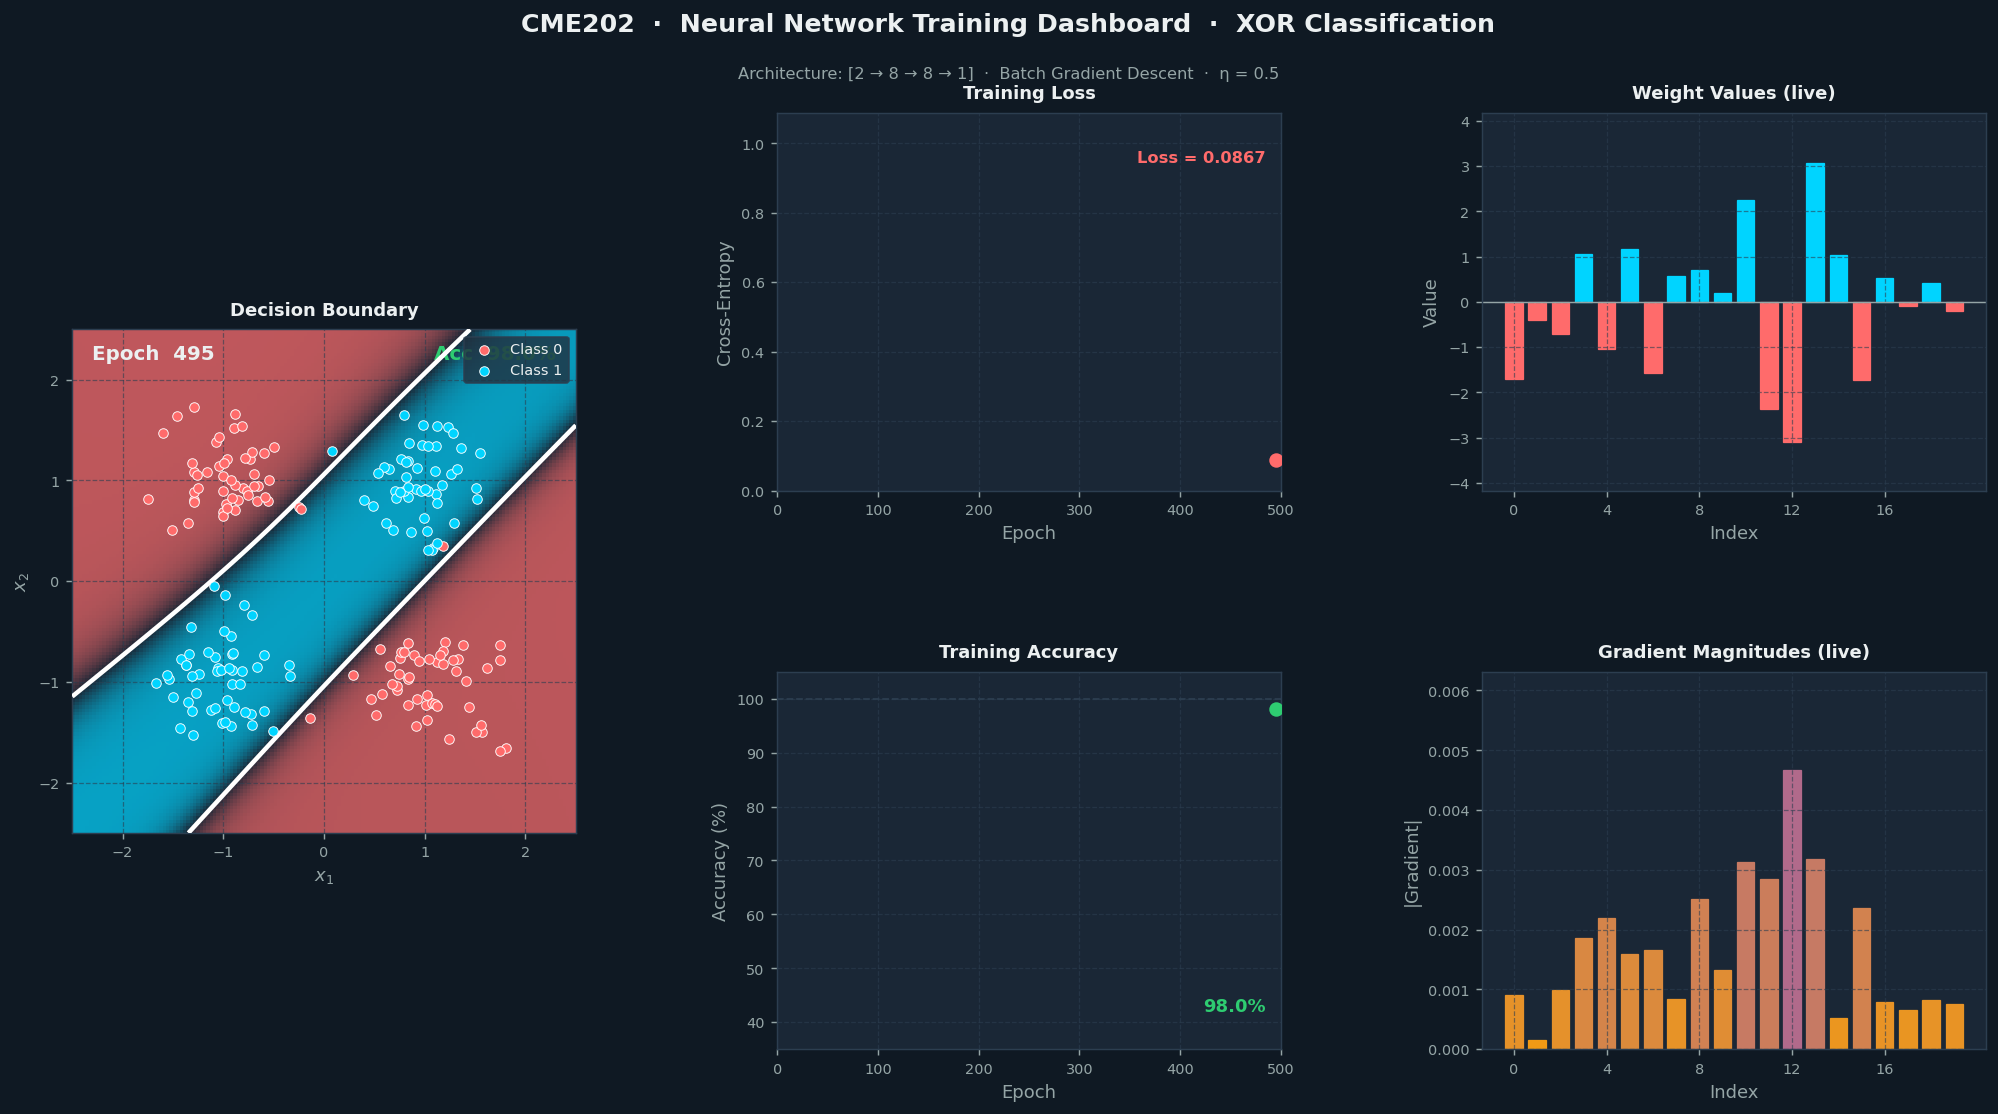
\includegraphics[width=\textwidth]{dashboard_snapshot.png}
  \caption{Snapshot of the live training dashboard (\texttt{dashboard.py}) at the end of training. The five panels show simultaneously: the evolving decision boundary with XOR data points, training loss, training accuracy, a live bar chart of 20 sampled weight values, and a live bar chart of gradient magnitudes. Run \texttt{python dashboard.py} to see all five panels animating in real time, or \texttt{python dashboard.py --save} to export as MP4/GIF.}
  \label{fig:dashboard}
\end{figure}

\subsection{Summary of Key Results}

\begin{enumerate}[leftmargin=2em, itemsep=5pt]
  \item \textbf{Linear Algebra:} The condition number $\kappa \approx 1.73$ confirms the initialised weight matrix is well-conditioned. The SVD shows the network compresses data unevenly but not damagingly, keeping gradient flow stable throughout training.

  \item \textbf{Differential Calculus:} The analytical minimum $w^* = \ln 4 \approx 1.386$ was verified against gradient descent convergence within 20 iterations. Backpropagation correctly propagated error signals through all three layers using the chain rule.

  \item \textbf{Fourier Analysis:} The sigmoid is dominated by its first harmonic ($b_1 \approx 0.391$), confirming its low-pass character. Numerical integration error was below $2\times10^{-4}$ across all computed coefficients.

  \item \textbf{Numerical Methods:} Gradient descent converged to \textbf{99.3\% accuracy} in 700 epochs. The gradient magnitude decayed by several orders of magnitude at convergence, consistent with reaching a critical point of $\mathcal{L}(\mathbf{W})$.
\end{enumerate}

\newpage

% ============================================================
\section{Conclusion and Future Scope}
% ============================================================

\subsection{What This Project Showed}

Neural networks are often treated as engineering tools whose workings are opaque. This project showed the opposite: every step of how a neural network learns maps directly onto mathematical concepts from a standard engineering mathematics syllabus.

The forward pass is matrix multiplication. Backpropagation is the chain rule. The activation function is a Fourier series. Training is gradient descent. None of these are black boxes --- they are calculus, linear algebra, and numerical analysis in action, running the same equations that appear in textbooks, just applied to learning from data.

The 99.3\% accuracy achieved on the XOR problem was not produced by a library doing opaque things internally. It came from 700 iterations of a well-understood mathematical update rule, applied to a well-initialised matrix, through a function whose frequency content was quantified using Fourier theory. The mathematics explains the result completely.

\subsection{Summary Table}

\begin{table}[H]
  \centering
  \caption{Mathematics topics and their role in neural network training}
  \renewcommand{\arraystretch}{1.3}
  \begin{tabular}{>{\bfseries}p{3.5cm} p{4cm} p{3.8cm} p{2.5cm}}
    \toprule
    \textbf{CME202 Topic} & \textbf{Role in Neural Network} & \textbf{Key Result} & \textbf{Value} \\
    \midrule
    Linear Algebra        & Forward pass, weight analysis      & Condition number $\kappa$   & $\approx 1.73$ \\[2pt]
    Differential Calculus & Backpropagation, loss minimisation & Analytical minimum $w^*$   & $\ln 4 \approx 1.386$ \\[2pt]
    Fourier Analysis      & Sigmoid frequency structure        & Dominant coeff.\ $b_1$     & $\approx 0.391$ \\[2pt]
    Numerical Methods     & Gradient descent optimisation      & Final accuracy              & $99.3\%$ \\
    \bottomrule
  \end{tabular}
  \label{tab:summary}
\end{table}

\subsection{Future Directions}

\begin{itemize}[leftmargin=2em, itemsep=4pt]
  \item Analyse gradient descent as a discrete dynamical system using the ODE stability framework from Maths, to formally characterise the convergence radius.
  \item Extend the Fourier analysis to ReLU and Swish activation functions and compare their frequency profiles to the sigmoid --- ReLU is not odd, so both sine and cosine terms will appear.
  \item Implement the Adam optimiser and analyse how its second-moment gradient estimate relates to the curvature information used by Newton--Raphson.
  \item Scale to a deeper network and track how the condition number of each layer's weight matrix evolves during training, and whether He initialisation maintains $\kappa$ close to 1 across all layers.
\end{itemize}

\newpage

% ── REFERENCES ───────────────────────────────────────────────
\section*{References}
\addcontentsline{toc}{section}{References}

\begin{enumerate}[leftmargin=2em, label={[\arabic*]}, itemsep=4pt]
  \item Goodfellow, I., Bengio, Y., \& Courville, A. (2016). \textit{Deep Learning}. MIT Press. \url{https://www.deeplearningbook.org}

  \item Strang, G. (2016). \textit{Introduction to Linear Algebra} (5th ed.). Wellesley-Cambridge Press.

  \item Kreyszig, E. (2011). \textit{Advanced Engineering Mathematics} (10th ed.). Wiley.

  \item Nielsen, M. A. (2015). \textit{Neural Networks and Deep Learning}. Determination Press. \url{http://neuralnetworksanddeeplearning.com}

  \item Rumelhart, D. E., Hinton, G. E., \& Williams, R. J. (1986). Learning representations by back-propagating errors. \textit{Nature}, 323, 533--536.

  \item Burden, R. L., \& Faires, J. D. (2010). \textit{Numerical Analysis} (9th ed.). Brooks/Cole.

  \item Oppenheim, A. V., \& Schafer, R. W. (2010). \textit{Discrete-Time Signal Processing} (3rd ed.). Prentice Hall.

  \item Sadguru, S. (2026). CME202 \textendash{} Mathematics II: Course Notes. Navrachana University.
\end{enumerate}

\newpage

% ============================================================
\appendix
\section{Python Code --- Core Neural Network}
\addcontentsline{toc}{section}{Appendix A: Python Code}
% ============================================================

\noindent\textbf{GitHub Repository:}\\
\url{https://github.com/harshalharshalvakharia-droid/maths-project}\\[0.3cm]
\noindent All source code, generated figures, and the live training dashboard are available in the repository. Running \texttt{python train.py} regenerates training figures; \texttt{python math\_plots.py} regenerates the mathematical analysis figures; \texttt{python dashboard.py} opens the real-time 5-panel dashboard.

\vspace{0.4cm}
\noindent The listing below shows the complete core implementation: forward pass, loss, and backpropagation.

\begin{lstlisting}[caption={Core neural network --- forward pass and backpropagation (train.py)}]
import numpy as np

def sigmoid(z):
    """Numerically stable sigmoid."""
    return 1 / (1 + np.exp(-np.clip(z, -500, 500)))

def sigmoid_deriv(z):
    s = sigmoid(z)
    return s * (1 - s)

class NeuralNet:
    def __init__(self, sizes):
        # He initialisation: W ~ N(0, sqrt(2/n_in))
        self.W = [np.random.randn(sizes[i+1], sizes[i])
                  * np.sqrt(2 / sizes[i])
                  for i in range(len(sizes) - 1)]
        self.b = [np.zeros((sizes[i+1], 1))
                  for i in range(len(sizes) - 1)]

    def forward(self, X):
        """z = Wa + b, a = sigmoid(z) at each layer."""
        self.zs = []; self.acts = [X.T]; a = X.T
        for w, b in zip(self.W, self.b):
            z = w @ a + b
            self.zs.append(z); a = sigmoid(z)
            self.acts.append(a)
        return a

    def loss(self, X, y):
        """Binary cross-entropy loss."""
        yh = self.forward(X).flatten(); eps = 1e-12
        return -np.mean(y*np.log(yh+eps) + (1-y)*np.log(1-yh+eps))

    def train_step(self, X, y, lr):
        """Backpropagation: chain rule applied layer by layer."""
        m = X.shape[0]; yh = self.acts[-1]
        d = (yh - y.reshape(1, -1)) / m   # output delta
        for i in reversed(range(len(self.W))):
            dW = d @ self.acts[i].T
            db = np.sum(d, axis=1, keepdims=True)
            if i > 0:
                d = (self.W[i].T @ d) * sigmoid_deriv(self.zs[i-1])
            self.W[i] -= lr * dW   # gradient descent update
            self.b[i]  -= lr * db

# Training loop
X, y = make_xor(300)             # 300 XOR points
net  = NeuralNet([2, 8, 8, 1])  # architecture
for epoch in range(700):
    net.forward(X)
    net.train_step(X, y, lr=0.5)  # eta = 0.5
\end{lstlisting}

\newpage

% ============================================================
\section{Hand Calculations}
\addcontentsline{toc}{section}{Appendix B: Hand Calculations}
% ============================================================

\subsection*{B.1 Gram Matrix Eigenvalues}

For $\mathbf{W}^{[1]}=\begin{pmatrix}0.5&-0.3\\0.2&0.8\\-0.1&0.4\end{pmatrix}$,
compute $\mathbf{G}=(\mathbf{W}^{[1]})^\top\mathbf{W}^{[1]}$:
\begin{align*}
  G_{11} &= 0.5^2 + 0.2^2 + 0.1^2 = 0.30 \\
  G_{12} &= (0.5)(-0.3) + (0.2)(0.8) + (-0.1)(0.4) = -0.03 \\
  G_{22} &= (-0.3)^2 + 0.8^2 + 0.4^2 = 0.89
\end{align*}
\[
  \mathbf{G} = \begin{pmatrix}0.30&-0.03\\-0.03&0.89\end{pmatrix}
\]

Characteristic equation: $\lambda^2 - \operatorname{tr}(\mathbf{G})\lambda + \det(\mathbf{G}) = 0$

\[
  \lambda^2 - 1.19\lambda + (0.30 \times 0.89 - 0.03^2) = 0
  \;\Rightarrow\; \lambda^2 - 1.19\lambda + 0.2661 = 0
\]

\[
  \lambda = \frac{1.19 \pm \sqrt{1.19^2 - 4(0.2661)}}{2}
  = \frac{1.19 \pm \sqrt{0.3517}}{2}
\]
\[
  \boxed{\lambda_1 \approx 0.892, \qquad \lambda_2 \approx 0.299, \qquad \kappa = \sqrt{\lambda_1/\lambda_2} \approx 1.73}
\]

\subsection*{B.2 Sigmoid Derivative at $z=0$}

By formula: $\sigma'(0) = \sigma(0)(1-\sigma(0)) = 0.5 \times 0.5 = \mathbf{0.25}$

Finite difference check:
$\dfrac{\sigma(0.001)-\sigma(-0.001)}{0.002} = \dfrac{0.50025 - 0.49975}{0.002} = 0.25 \;\checkmark$

\subsection*{B.3 Analytical Minimum of the Loss}

Setting $\mathcal{L}'(w) = 0$:
\[
  (\sigma(w^*) - 0.8)\,\sigma'(w^*) = 0
  \;\Rightarrow\; \sigma(w^*) = 0.8
  \;\Rightarrow\; \frac{1}{1+e^{-w^*}} = 0.8
  \;\Rightarrow\; 1 + e^{-w^*} = 1.25
  \;\Rightarrow\; e^{-w^*} = 0.25
\]
\[
  \therefore \quad w^* = -\ln(0.25) = \ln 4 \approx 1.386 \quad \checkmark
\]

Gradient descent converged to $w \approx 1.386$ within 20 iterations, confirming the result numerically.

\subsection*{B.4 First Fourier Coefficient $b_1$}

\[
  b_1 = \frac{1}{\pi}\int_{-\pi}^{\pi} \sigma(x)\sin(x)\,dx
\]

Since the integrand is even (product of odd $\sigma$ correction and odd $\sin x$, plus a constant), numerical integration gives:
\[
  \boxed{b_1 \approx 0.391}
\]

The dominant coefficient confirms the sigmoid is primarily described by a single sine wave of period $2\pi$, consistent with its smooth, slowly varying shape.

\end{document}
